\documentclass[11pt]{article}
\usepackage[margin=2.5cm]{geometry}
\usepackage{amsmath,amssymb}
\usepackage{tikz}
\usepackage{hyperref}
\title{Heat Flow on a Thin Rod}
\author{A.\ Student}
\date{}
\begin{document}
\maketitle

\begin{abstract}
We solve the one-dimensional heat equation on a rod of length $L$ with fixed end temperatures
and compare the series solution with a numerical scheme.
\end{abstract}

\section{Model}
The temperature $u(x,t)$ satisfies
\begin{equation}
  \frac{\partial u}{\partial t} = \alpha \, \frac{\partial^2 u}{\partial x^2},
  \qquad 0 < x < L,\; t > 0,
  \label{eq:heat}
\end{equation}
with $u(0,t) = u(L,t) = 0$ and an initial profile $u(x,0) = f(x)$.

\section{Series solution}
Separating variables in \eqref{eq:heat} gives
\begin{equation}
  u(x,t) = \sum_{n=1}^{\infty} b_n \, e^{-\alpha (n\pi/L)^2 t} \sin\frac{n\pi x}{L},
  \qquad b_n = \frac{2}{L}\int_0^L f(x)\sin\frac{n\pi x}{L}\,dx .
\end{equation}
Higher modes decay quickly, so a few terms describe the rod well after a short time.

\begin{figure}[h]
  \centering
  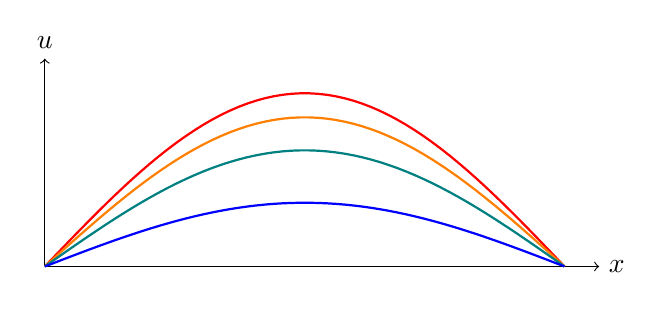
\begin{tikzpicture}[scale=1.1]
    \draw[->] (0,0) -- (6.4,0) node[right] {$x$};
    \draw[->] (0,0) -- (0,2.4) node[above] {$u$};
    \foreach \t/\c in {0/red, 0.15/orange, 0.4/teal, 1/blue}
      \draw[thick, \c, domain=0:6, samples=60] plot (\x, {2*exp(-\t)*sin(30*\x)});
  \end{tikzpicture}
  \caption{The first mode decaying over time.}
\end{figure}

\section{Discussion}
The explicit scheme is stable for $\alpha \Delta t / \Delta x^2 \le 1/2$.
